\documentclass[10pt,portuguese]{article}

\usepackage{fourier}

\usepackage[]{graphicx}
\usepackage[]{color}
\usepackage{xcolor}
\usepackage{alltt}
\usepackage{listings}
\usepackage[T1]{fontenc}
\usepackage[utf8]{inputenc}
\setlength{\parskip}{\smallskipamount}
\setlength{\parindent}{5ex}
\usepackage{indentfirst}
\usepackage{listings}
\usepackage{setspace}
\usepackage{hyperref}
\definecolor{blue(munsell)}{rgb}{0.0, 0.5, 0.69}
\hypersetup{
    colorlinks=true,
    linkcolor=auburn,
    filecolor=magenta,      
    urlcolor=blue, urlsize=2em
}

% Set page margins
\usepackage[top=100pt,bottom=100pt,left=68pt,right=66pt]{geometry}

% Package used for placeholder text
\usepackage{lipsum}

% Prevents LaTeX from filling out a page to the bottom
\raggedbottom


\usepackage{fancyhdr}
\fancyhf{} 
\fancyfoot[C]{\thepage}
\renewcommand{\headrulewidth}{0pt} 
\pagestyle{fancy}

\usepackage{titlesec}
\titleformat{\chapter}
   {\normalfont\LARGE\bfseries}{\thechapter.}{1em}{}
\titlespacing{\chapter}{0pt}{50pt}{2\baselineskip}

\usepackage{float}
\floatstyle{plaintop}
\restylefloat{table}

\usepackage[tableposition=top]{caption}



\frontmatter

\definecolor{light-gray}{gray}{0.95}

\renewcommand{\contentsname}{Table of Contents}

\begin{document}


\begin{titlepage}
	\clearpage\thispagestyle{empty}
	\centering
	\vspace{2cm}

	
	{\Large\underline{Inteligência Artificial} \par}
	\vspace{0.5cm}
	{\small
	Diogo Nuno Pereira Gomes \par Luís Filipe de Seabra Lopes  \par}
	\vspace{4cm}
	{\LARGE \textbf{Sokoban Solver}} \\
		\vspace{0.5cm}
	\vspace{1cm}
	\vspace{4cm}
	{\normalsize Hugo Paiva, 93195
	        \\Carolina Araújo, 93248
	   \par}
	\vspace{2cm}

    
\includegraphics[scale=0.20]{logo_ua.png}
    
    \vspace{2cm}
    
	{\normalsize DETI \\ 
		Universidade de Aveiro \par}
		
	{\normalsize 11-12-2020 \par}
	\vspace{2cm}
		
	
	\pagebreak

\end{titlepage}
\newpage

\section{Introdução}

\par Este trabalho prático foi desenvolvido com o objetivo de implementar um \textbf{agente inteligente} capaz de resolver diversos níveis do jogo \textbf{Sokoban}, sem necessitar de conhecimento \textit{a priori} dos mesmos. 

\section{Arquitetura}
\par A solução desenvolvida utiliza o \textit{solver} de problemas do Standford Research Institute (\textbf{STRIPS}), que é uma técnica de planeamento automático, descrevendo primeiro o mundo. Isto é feito fornecendo objetos, ações, pré-condições e efeitos. 

\par A imagem seguinte fornece uma ideia geral de toda a implementação:

    \begin{figure}[!h]
        \centering
        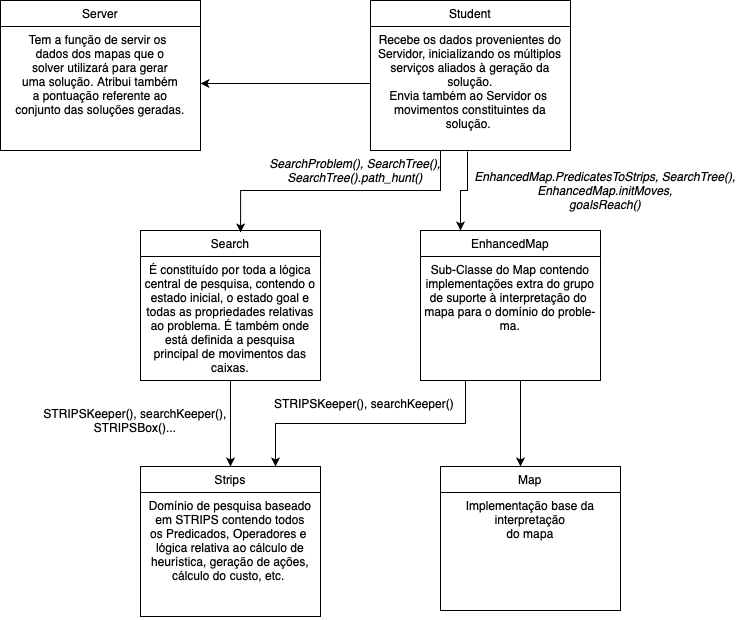
\includegraphics[width=291]{d_diagram.png}
        \caption{Arquitetura do trabalho prático desenvolvido} 
    \end{figure}


\section{Sokoban Solver}
\par Inicialmente o grupo debruçou-se sobre a pesquisa de quais os movimentos possíveis em cada posição do mapa, bem como a pesquisa de um caminho desde a posição do \textit{keeper} até uma determinada caixa. Com isto foi possível avançar o suficiente para se chegar a níveis onde não se encontrava a tempo uma solução, visto que muitas das possibilidades que estavam a ser exploradas entravam em situação de \textit{deadlock}. O próximo passo foi, então, prevenir o contínuo estudo de jogadas impossíveis, pelo que se implementaram funções para detetar \href{http://sokobano.de/wiki/index.php?title=How_to_detect_deadlocks}{\textit{deadlocks}}, como \textit{simple deadlocks}, \textit{freeze deadlocks} e \href{http://www.sokobano.de/wiki/index.php?title=Deadlocks}{\textit{dead square deadlocks}}. 
\par Com isto, foi possível atingir patamares muito mais elevados, quando os algoritmos de deteção de \textit{deadlocks} estavam já aprumados, no entanto faltava otimização. A título de exemplo, um dos erros, por assim dizer, cometido a ínicio, e que estava a atrasar bastante o processo de pesquisa, era o facto apenas se estar a verificar a existência de um determinado nó em todos os seus nós superiores até à raiz. Ao fazer isto, estavam-se a calcular múltiplos estados já calculados previamente. A solução foi utilizar um \textit{set} para guardar todos os estados já criados.
\par Algo também muito batalhado foi a escolha da heurística para o cálculo estimado do tamanho do caminho desde uma caixa até um \textit{goal}. Várias implementações foram exploradas, uma delas envolvendo a própria pesquisa de um caminho desde a caixa até um goal, o que demorava demasiado tempo, pelo que o grupo acabou por escolher outra implementação. Aqui considerava-se que eram prioritários os estados onde mais caixas se encontrassem já em \textit{goals}, bem como os estados onde as caixas já se encontravam na mesma linha ou coluna que os \textit{goals}. Quanto à heurística usada na pesquisa dos caminhos das caixas até aos \textit{goals}, escolheu-se uma simples que calculava a \href{https://pt.wikipedia.org/wiki/Geometria_pombalina}{distância de Manhattan}, em vez da \href{https://pt.wikipedia.org/wiki/Dist\%C3\%A2ncia_euclidiana}{distância Euclidiana}, visto que a primeira, embora não tenha em consideração paredes e caixas que possam estar no caminho, e, por isso, provocar desvios, é mais realista do que a distância linear entre os pontos, visto que o \textit{keeper} nem pode andar na diagonal.
\par É de notar que a explicação de todos os algoritmos se encontra em forma de comentário no código, facilitando não só a leitura do mesmo mas também o raciocínio por detrás de algumas das escolhas feitas.




\section{Estratégia de Validação da Solução}
\par Em termos de validação da solução, eram realizadas propostas de algoritmos que facilitassem a pesquisa e colocava-se a correr o programa, por vezes num nível em concreto, e, com base na medição do tempo que cada parte do código demorava, era possível chegar a diferentes conclusões, \textit{i.e}, havia uma melhor perceção de qual o excerto de código que poderia estar a causar problemas. Com base nisto, eram realizadas otimizações, como por exemplo garantir que apenas era realizada a quantidade estritamente necessária de ciclos \textit{for} e \textit{while}, que não eram realizadas chamadas a funções fundamentais e que pudessem ser substituídas por outra solução mais direta, \textit{etc}. 
\par Usava-se, também, a tabela fornecida pelos docentes como forma de entender onde o grupo se encontrava em comparação com outros grupos, e, portanto, o quão próximos estariamos de uma solução plausível. 

\subsubsection{Estatística}

\par Com o objetivo de analisar os resultados do trabalho prático, foram gerados dados relativos ao processamento de cada solução de modo a possibilitar a criação de gráficos. A implementação desta geração de dados encontra-se na \textit{branch} \textit{generate\_graph\_data}.

\par Apesar de os dados terem sido gerados, devido à escassez de tempo, não foi possível criar visualizações dos mesmos. Apesar disto, os dados encontram-se na pasta \textit{stats} do repositório.

\section{Conclusão}
\par Em tom de remate, de acordo com as metas especificadas pelos docentes, pensa-se que o trabalho foi bem sucedido. Uma das dificuldades mais sentidas pelo grupo foi perceber o que podia estar a impedir que fosse possível encontrar uma solução antes de se ocorrer \textit{timeout} e quais os \textit{deadlocks}, ou outros pequenos pormenores, que podiam estar a interferir com o tempo que demorava a pesquisar por uma solução. Pensa-se ter alcançado bons resultados, visto que é possível passar com sucesso todos os níveis até ao 130, inclusive.
\par Considera-se que este trabalho prático ajudou a aprofundar  conhecimento prévio sobre estruturas de dados e quais os tipos de pesquisa que é possível realizar sobre as mesmas, nomeadamente em árvores, bem como adquirir novos conhecimentos relacionados.
\par Todavia, o grupo considera que, embora se considere que tenham sido obtidos bons resultados, a primeira entrega não correu como esperado, sendo que se desejava ter conseguido solucionar mais níveis. Ainda assim, pensa-se que a evolução entre a primeira e a segunda entrega foi notável e já demonstrou melhor o empenho e tempo que foram colocados no trabalho. 

\section{Referências}

\par Foi interpretada bastante informação relativa aos problemas e métodos de solução do \textit{Sokoban} através de artigos e relatórios de estudos encontrados na internet. No entanto, para toda a implementação mais importante foi usada como base de pesquisa a \href{http://sokobano.de/wiki/index.php?title=Solver}{\textit{Sokoban Wiki}}.

\par A nível de otimização de código, consoante o que o grupo verificava que estava a usar mais tempo de processamento foram sendo pesquisadas diversas soluções. A implementação de \href{https://docs.python.org/3/library/heapq.html}{\textit{Heap}} em \textit{Python} é um dos exemplos do resultado destas pesquisas.

\par Foram debatidas ideias com o grupo do aluno Lucas Botto 93019, e Rui Fernandes 92952. \end{document}

